\question[10] Sofía arma cuadrados con fósforos. En la siguiente imagen, hay tres figuras que Sofía armó:

\begin{minipage}{0.4\linewidth}
    \begin{figure}[H]
        \centering
        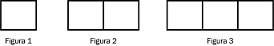
\includegraphics[width=0.9\textwidth]{../images/9b2788ac343174f7bbf340e98582d00a42c4804d}
        \caption{Ilustración de los bloques de plástico}
        \label{fig:9b2788ac343174f7bbf340e98582d00a42c4804d}
    \end{figure}
\end{minipage}\hfill
\begin{minipage}{0.6\linewidth}
    Sofía observa esta secuencia de figuras y dice:

    Si sigo armando cuadrados según esta secuencia, al terminar de armar la Figura \ref{9b2788ac343174f7bbf340e98582d00a42c4804d}, habré utilizado menos de 640 fósforos.
    \textbf{¿Es correcto lo que dice Sofía? ¿Por qué?}
\end{minipage}


